\documentclass[12pt,a4paper]{report}
\usepackage[utf8]{inputenc}
\usepackage[francais]{babel}
\usepackage[T1]{fontenc}
\usepackage{amsmath}
\usepackage{amsfonts}
\usepackage{amssymb}
\usepackage{url}
\usepackage{ucs}
\usepackage{graphicx}
\usepackage{lmodern}
\usepackage{xcolor}
\usepackage[left=2cm,right=2cm,top=2cm,bottom=2cm]{geometry}
\author{Typhaine PL}
\setcounter{tocdepth}{1} 
\usepackage{lmodern}

\makeatletter
\def\clap#1{\hbox to 0pt{\hss #1\hss}}%
\def\ligne#1{%
\hbox to \hsize{%
\vbox{\centering #1}}}%
\def\haut#1#2#3{%
\hbox to \hsize{%
\rlap{\vtop{\raggedright #1}}%
\hss
\clap{\vtop{\centering #2}}%
\hss
\llap{\vtop{\raggedleft #3}}}}%
\def\bas#1#2#3{%
\hbox to \hsize{%
\rlap{\vbox{\raggedright #1}}%
\hss
\clap{\vbox{\centering #2}}%
\hss
\llap{\vbox{\raggedleft #3}}}}%
\def\maketitle{%
\thispagestyle{empty}\vbox to \vsize{%
\haut{}{\@blurb}{}
\vfill
\vspace{1cm}
\begin{flushleft}
\usefont{OT1}{ptm}{m}{n}
\huge \@title
\end{flushleft}
\par
\hrule height 4pt
\par
\begin{flushright}
\usefont{OT1}{phv}{m}{n}
\Large \@author
\par
\end{flushright}
\vspace{1cm}
\vfill
\begin{center}
\includegraphics[width=0.3\textwidth]{../Images/logo/logo.png}\\
\vspace{2cm}
\includegraphics[width=0.1\textwidth]{../Images/logounibdx.png}
\end{center}
\vfill
\bas{}{\@date}{}
}%
\cleardoublepage
}
\def\date#1{\def\@date{#1}}
\def\author#1{\def\@author{#1}}
\def\title#1{\def\@title{#1}}
\def\location#1{\def\@location{#1}}
\def\blurb#1{\def\@blurb{#1}}
\date{\today}
\author{}
\title{}
\location{}\blurb{}
\makeatother
\title{Conception d'un Projet de Recherche}
\author{\textsc{FR\`ECHE} Arnaud, \textsc{H\'ERIC\'E} Charlotte, \textsc{MOLA} Saraï,\\ \textsc{PAYSAN-LAFOSSE} Typhaine, \textsc{SANSEN} Joris}
\location{Bordeaux}
\blurb{%
Universités de Bordeaux\\
Master 2 BioInformatique
\textbf{}\\[1em]
\textsc{Marie Beurton Aimar}
}%
\begin{document}
\maketitle
\tableofcontents
\chapter*{Introduction}

\chapter{Analyse}

%%%%%%%%%%%%%%%%%%%%%%%%%%%%%%
\chapter{Contexte}
%%%%%%%%%%%%%%%%%%%%%%%%%%%%%%
Le métabolisme d'une cellule est un système complexe de transformations moléculaires et énergétiques qui se déroulent 
de manière ininterrompue dans la cellule et mettant en jeu un ensemble de réactions dites métaboliques. 
Ces réactions impliques différents types de métabolites qui, suivant leurs positions dans la réaction, sont appelées substrats 
ou produits et sont généralement catalysées par des enzymes.

Afin de faciliter leurs études, on associe un ensemble de ces réactions métaboliques de façon à représenter les grandes 
fonctions métaboliques (glycolyse, etc) créant ainsi des réseaux métaboliques. Cette modélisation de réactions permet 
de réaliser des requêtes complexes comme, par exemple, le calcul (et la prédiction) de tous les métabolites pouvant 
être générés à partir d’un ensemble de composés sources.

Quelques logiciels disponibles internationalement permettent de travailler et d'automatiser l'étude de ces réseaux et proposent 
des outils tels que le calcul des modes élémentaires de flux ou la recherche de minimal \textit{cut sets}. 
Cependant, ils sont soit dépendants de logiciels non libre comme MATLAB, soit ne possèdent pas d'interface utilisateur conviviale.\\

\pagebreak
%%%%%%%%%%%%%%%%%%%%%%%%%%%%%%
\chapter{État de l'existant}
%%%%%%%%%%%%%%%%%%%%%%%%%%%%%%

\section{Efmtool}

Efmtool calcule les modes élémentaires de flux de réseaux métaboliques. Il est implémenté en Java et a été intégré à MATLAB.\\
Il a été développé par Marco Terzer. La version courante est la 4.7.1 (Décembre 2009).

\section{\emph{RegEfmtool}}

\emph{RegEfmtool} est un outil informatique qui combine le calcul des modes élémentaires de flux et la régulation transcriptionnelle du réseau métabolique. Il a été développé, entre autres, par Christian Jungreuthmayer. Il a été créé afin d'accélérer le calcul de jeux complets de modes élémentaires de flux d'un réseau métabolique.\\
\emph{RegEfmtool} est une extension d'Efmtool qui prend en compte la régulation transcriptionnelle des réseaux pour le calcul des modes élémentaires de flux.\\
La prise en compte de la régulation des gènes réduit de façon importante le nombre de solutions et permet d'éliminer constamment les modes qui ne peuvent exister biologiquement pendant et après le processus de calcul. Elle permet aussi de réduire considérablement le coût du calcul.\\
L'installation et l'utilisation de \emph{regEfmtool} a été exclusivement testée sous Linux. Elle pourrait cependant fonctionner sous d'autres systèmes d'exploitation puisqu'il s'agit d'un programme Java. Il n'existe pas d'interface graphique de cette application, elle s'exécute donc en lignes de commandes via le terminal.
La version courante de \emph{RegEfmtool} est la 2.0 (Août 2012).

\section{METATOOL} 

METATOOL est un programme écrit en C développé de 1998 à 2000 par Thomas Pfeiffer (Berlin) en coopération avec Juan Carlos Nuno (Madrid), Stefan Schuster (Berlin) et Ferdinand Moldenhauer (Berlin).\\
Il sert à étudier la structure des réseaux métaboliques à partir d'équations de réactions stœchiométriques et permet notamment de calculer les modes élémentaires.\\
Les premières versions de METATOOL (jusqu'à la 4.9) ont été développées en C. Aujourd'hui, nous trouvons aussi une version de METATOOL en C++ mais cette version n'est pas au point. La dernière version, 4.9, est assez performante sur les petits réseaux métaboliques, mais possède de gros problèmes de gestion de mémoire et de rapidité lors de calculs sur de grands réseaux.
Dans la version actuelle (5.1) l'exécutable est désormais un module de MATLAB 7 et GNU 3.0 Octave, il se présente sous la forme d'un ensemble de fichiers scripts de MATLAB.\\

Les paramètres donnés en entrée pour le bon fonctionnement du logiciel METATOOL sont les suivants:
\begin{enumerate}
\item la liste des réactions réversibles, ainsi que celle des réactions irréversibles, avec le nom des réactions,
\item la liste des métabolites internes et externes impliqués dans les réactions,
\item les équations réactionnelles se trouvant dans la section.
\end{enumerate}
Le tout est rassemblé dans un fichier avec l'extension \textit{.dat}\\

A la fin de son exécution, METATOOL a généré un fichier avec l'extension \textit{.out} dans lequel se trouvent les résultats. Dans les versions de METATOOL écrites en C, le fichier de sortie contient l'ensemble des résultats sous forme de matrices, ainsi que des bilans qui permettent de décrire le réseau d'étude.\\
Les versions de METATOOL écrites en MATLAB produisent des résultats similaires en terme de calcul des matrices des modes élémentaires mais les résultats sont disposés différemment dans le fichier de sortie.

\section{CellNetAnalyzer}

CellNetAnalyzer est un package de MATLAB (écrit en \textsc{C}) qui fourni un environnement compréhensible et convivial pour l'utilisateur et qui permet une analyse fonctionnelle et structurelle de réseaux biochimiques. Il a été développé à l'institut Max Planck de Magdeburg par Steffen Klamt (depuis 2000) et Axel von Kamp (depuis 2007) notamment.\\
CellNetAnalyzer fourni une importante collection d'outils et d'algorithmes pour l'analyse structurelle de réseaux.\\
C'est un programme gratuit pour une utilisation académique. Pour l'exécuter, il faut avoir installé MATLAB 7.0 ou une version ultérieure qui demande une licence. Il peut être utilisé sur Linux, Windows XP ou Mac.\\
Pour l'étude des modes élémentaires, CellNetAnalyzer fait appel à METATOOL via le logiciel MEX qui sert d'interface. MEX permet à MATLAB d'appeler tout logiciel \textsc{C} externe pour compléter les outils qu'il possède.

\section{Langages}

Notre projet nécessite l'utilisation d'une interface web, dans ce cadre il existe:
\begin{itemize}
\item \textsc{mod perl} combiné avec \textsc{apache} et \textsc{CGI} mais la technologie utilisée est à l'heure actuelle dépassée
\item \textsc{mod python} combiné avec \textsc{apache} et \textsc{CGI} mais même remarque que précédemment
\item \textsc{CL-WHO} avec \textsc{Hunchentoot} et \textsc{ParenScript} offre un bon environnement pour le développement web
\item \textsc{Java} et ses \textsc{applets java} apparaissent également comme un bon choix pour le développent web
\item \textsc{PHP} couplé avec du \textsc{Javascript} peut être un choix judicieux pour une application web\\
\end{itemize}

Parmi les différents choix précédemment cités, deux sortent du lot: \textsc{Java} et \textsc{PHP} avec leurs bibliothèques.
\pagebreak
%%%%%%%%%%%%%%%%%%%%%%%%%%%%%%
\section{Analyse des besoins}
%%%%%%%%%%%%%%%%%%%%%%%%%%%%%%

\subsection{Besoins fonctionnels}

\subsubsection{Interface Homme Machine (IHM)}
L'interface Web que nous avons réalisé permet de charger la description d'un réseau pré-existant ou d'en créer un nouveau.\\
Elle donne également le moyen à l'utilisateur de saisir les fonctions et options qui l'intéressent puis de lancer les calculs des modes élémentaires de flux du réseau d'intérêt. 

\subsubsection{Chargement des données}
Une zone de chargement de fichiers à partir du disque dur de l'utilisateur est présente sur l'interface. 
%Selon le type du fichier donné en paramètre d'entrée, une liste de choix possibles pourra être proposée. Ainsi les résultats d'expériences similaires (suppression, modification des réactifs, produits ou enzymes du réseau) devront pouvoir être comparés avec un affichage en vis-à-vis, ce qui implique une sauvegarde temporaire des résultats sur le serveur. 

\subsubsection{Réglage des paramètres}
Il est possible pour un utilisateur confirmé ou habitué à l'interface d'avoir accès à un mode de réglage avancé des paramètres, s'il le désire. Ces derniers sont fixés à des valeurs par défaut pour les débutants. 

\subsubsection{Résultats}
Enfin, la visualisation des résultats apparaît de façon claire et conviviale à l'utilisateur au travers de l'interface Web. De plus, les résultats sont également présents dans des fichiers pour une analyse ultérieure. %Par ailleurs, nous allons essayer de mettre en place un dispositif d'annotations des fichiers.

\subsubsection{Aide en ligne}
Un message d'aide apparaît au survol du curseur de la souris sur la fonction ou l'option choisie. Ainsi l'utilisateur pourra avoir plus d'informations sur la commande concernée.\\
Des pages d'aide sont aussi consultable pour la création d'un nouveau réseau.\\

Lors de l'affichage de la page d'accueil, l'utilisateur aura le choix entre créer un réseau métabolique manuellement, ou bien le charger à partir de fichiers préexistant. 
			
\subsubsection{Création d'un nouveau réseau}

Si l'utilisateur clique sur le bouton de création d'un nouveau réseau métabolique, une première page Web s'affiche. Il peut alors initialiser les fichiers présents sur son disque dur et écrire les réactions qui composent son réseau. Il a aussi la possibilité de modifier une réaction (métabolites, coefficients stœchiométriques). Lorsqu'il ajoute ou modifie une réaction, les données sont récupérées afin de générer automatiquement les fichiers nécessaires au fonctionnement du logiciel.
L'utilisateur peut aussi générer un fichier \emph{DAT} s'il le désire.\\
Lorsqu'il choisi de passer à l'étape suivante, il peut créer les règles qui seront utilisées par \emph{regEfmtool} pour calculer les modes élémentaires.

\subsubsection{Chargement d'un réseau préexistant}

Si l'utilisateur clique sur le bouton de chargement d'un réseau depuis la page d'accueil, il doit sélectionner les options de lancement de la commande \emph{regEfmtool} puis charger une série de fichiers (depuis le disque dur de son ordinateur) nécessaires au bon fonctionnement du logiciel. %Les fichiers doivent être dans le format adéquat et un message d'erreur appara\^itra si ce n'est pas le cas. Au cas où, une fonction d'aide sera disponible pour avoir un modèle de fichiers à charger. 

\subsubsection{Lancement du programme}
Lorsque l'utilisateur aura créé son réseau manuellement ou l'aura chargé, il devra ensuite choisir les paramètres de calcul de \textit{regEfmtool}. Nous avons fait le choix d'utiliser des cases à cocher en fonction de ce qu'il choisira. Pour les utilisateurs non expérimentés, les choix de base seront pré-sélectionnés. Il suffira ensuite de cliquer sur le bouton "Lancement" pour avoir les résultats générés par le logiciel.

\subsubsection{Affichage des résultats}
A revoir!!!
%Il sera composé d'une série de "boîtes" dans lesquelles seront affichés les différents éléments générés par \textit{regEfmtool}. Il sera également possible de lancer une comparaison des résultats entre deux réseaux en appuyant sur le bouton "Compare". 

%\subsubsection{Comparaison des résultats}
%Pour la comparaison des réseaux, il y aura un affichage en vis-à-vis des résultats. 

\subsection{Besoins non fonctionnels}

\subsubsection{Portabilité}
L'utilisation de \textit{regEfmtool} s'appuie sur d'autres logiciels, nécessitant par exemple la version 1.7 de Java. De ce fait, ils devront être libre d'utilisation pour le secteur académique. L'interface devra être livrée avec tous les fichiers de configuration (pré-existants ou nouvellement créés) et indépendante du système d'exploitation. 

\subsubsection{Sécurité et robustesse}
Il faudra gérer l'espace occupé par les fichier chargés sur le serveur. Le site devra être stable et gérer au mieux les erreurs qui pourraient être générées lors du chargement des fichiers, de la modification des paramètres ou des calculs. %L'utilisateur sera donc informé en cas d'erreur lors du chargement d'un fichier non compatible avec \textit{regEfmtool}, contenant des erreurs d'écritures ou lorsque les paramètres entrés ne sont pas en accords avec la fonction ou l'option sélectionnée. 

%\subsubsection{Temps de calcul}
%Il faudra effectuer une vérification du nombre de métabolites et de réactions afin d'estimer le temps de calcul. Si ce dernier s'avère trop long, l'utilisateur sera prévenu et devra confirmer le lancement du processus. 

\subsubsection{Documentation}
L'écriture du code sera constituée de commentaires qui permettront la maintenance du code ainsi qu'une éventuelle amélioration de ce dernier par un tiers.
L'interface Web créée, quand à elle, devra être fournie avec une documentation sur son installation, son utilisation, sa maintenance et une charte graphique déclarant les différents attributs du site (couleurs utilisées, police, logo, image,...).


%%%%%%%%%%%%%%%%%%%%%%%%%%%%%%
\chapter{Conception}
%%%%%%%%%%%%%%%%%%%%%%%%%%%%%%

%~~~~~~~~~~~~~~~~~~~~~~~~~~~~~
\section{Interface graphique}
%~~~~~~~~~~~~~~~~~~~~~~~~~~~~~

Comme nous l'avons précisé précédemment, notre interface graphique se présente sous la forme d'un site Web. 

\begin{figure}[!ht]
	\begin{center}
		\fbox{
   		 \begin{minipage}[c]{0.9\textwidth}
  			\includegraphics[width=0.90\textwidth]{../Images/Rapport/pageAccueil.png}  
		 \end{minipage}}
		\caption{Page d'accueil}
  		\label{main}
  	\end{center}	
\end{figure}

Lorsqu'un utilisateur arrive sur le site, une page d'accueil s'affiche (Figure \ref{main}). Elle contient des informations relatives à l'utilisation du programme (à quoi il sert, que peut-on y faire ...). A partir de là, deux choix s'offrent à lui:
\begin{itemize}
\item Soit il créé un nouveau réseau, en cliquant sur \emph{Création} dans le menu situé en haut de page,
\item Soit il charge un réseau qu'il a déjà créé en cliquant sur \emph{Chargement}.\\
\end{itemize}

Chaque page du site se présente de la m\^eme façon: un menu en haut de la page et le logo du site Web dans un bandeau situé sur la gauche.\\
Le menu contient quatre onglets:
\begin{itemize}
\item \emph{Accueil} qui permet de retourner sur la page d'accueil du site Web,
\item \emph{Création} qui permet de créer un nouveau réseau métabolique,
\item \emph{Chargement} qui permet de charger un réseau pré-existant,
\item \emph{Aide} qui permet de consulter une aide à l'utilisation du site.
\end{itemize}
On trouve aussi dans le menu, trois drapeaux qui permettent de changer la langue du site Web. Les trois langues proposées sont: l'anglais, le français et l'allemand. Par défaut le site est en français.

%~~~~~~~~~~~~~~~~~~~~~~~~~~~~~
\section{Création d'un nouveau réseau}
%~~~~~~~~~~~~~~~~~~~~~~~~~~~~~

Si l'utilisateur choisi de créer un nouveau réseau, il arrive sur une page qui va lui permettre d'ajouter de nouvelles réactions à celui-ci. \\

Une première partie permet d'initialiser les fichiers (Figure \ref{creation1}) dans le cas où l'utilisateur aurait déjà créé un réseau précédemment.\\

\begin{figure}[!ht]
	\begin{center}
		\fbox{
   		 \begin{minipage}[c]{0.9\textwidth}
  			\includegraphics[width=0.90\textwidth]{../Images/Rapport/creation1.png}  
		 \end{minipage}}
		\caption{Page de création d'un nouveau réseau}
  		\label{creation1}
  	\end{center}	
\end{figure}

Une seconde partie permet de créer une nouvelle réaction. Celle-ci doit être de la forme $reaction : reag1 + reag2 => 2 prod1 + 4 prod2$. \\
L'utilisateur doit également préciser si la réaction est réversible ou non. Ensuite il clique sur le bouton \emph{Ajouter}, la réaction est alors ajoutée au réseau et apparaît dans la zone de texte située en-dessous. Dans cette zone de texte, l'utilisateur a la possibilité de modifier les réactions déjà créées (mais ne peut pas en ajouter ou en supprimer car les règles de réversibilités ne seraient alors pas respectées pour l'écriture d'un fichier au format \emph{DAT}). Il valide ensuite les modifications apportées en cliquant sur le bouton \emph{Modifier}.\\

\begin{figure}[!ht]
	\begin{center}
		\fbox{
   		 \begin{minipage}[c]{0.9\textwidth}
  			\includegraphics[width=0.90\textwidth]{../Images/Rapport/creation2.png}  
		 \end{minipage}}
		\caption{Suite de la page de création}
  		\label{creation2}
  	\end{center}	
\end{figure}

Enfin, l'utilisateur peut aussi générer un fichier au format \emph{DAT} (Figure \ref{creation2}) qui pourra être utilisé dans METATOOL par exemple.\\

\begin{figure}[!ht]
	\begin{center}
		\fbox{
   		 \begin{minipage}[c]{0.9\textwidth}
  			\includegraphics[width=0.90\textwidth]{../Images/Rapport/helpCreation.png}  
		 \end{minipage}}
		\caption{Page d'aide à la création d'un nouveau réseau}
  		\label{helpCreation}
  	\end{center}	
\end{figure}

Si l'utilisateur ne sait pas comment faire, il lui suffit de cliquer sur \textit{Aide} et une nouvelle fen\^etre de navigation (Figure \ref{helpCreation}) appara\^itra afin de la guider. Cette page est automatiquement traduite dans la langue de la page courante. 

Quand l'utilisateur a fini de créer toutes les réactions qui composent son réseau, il clique sur le bouton \emph{\'Etape suivante} et arrive alors sur la page de création des règles des gènes.

%~~~~~~~~~~~~~~~~~~~~~~~~~~~~~
\section{Règles des gènes}
%~~~~~~~~~~~~~~~~~~~~~~~~~~~~~

Ces règles sont utilisées pour éliminer les modes élémentaires non possibles dans un réseau métabolique réel.\\

Une réaction R peut \^etre 1-active (R=1), 0-active (R=0) ou encore full-active (R=f).\\
La création des règles est régie selon certains principes:
\begin{itemize}
\item La réaction de sortie ne peut jamais être une réaction d'entrée. \\On ne peut pas écrire: R3 = ( ! ( ( ! 0R3) $|$  1R1) )
\item Une réaction peut être utilisée plusieurs fois comme réaction d'entrée. \\Ex: R11 = ( ( ! ( ( ! 0R3) $|$ 1R5) ) \& 1R3)
\item Le préfixe d'une réaction n'est valable que pour une opération.\\ Ainsi dans la règle R11 = ( ( ! ( ( ! 0R3) $|$ 1R5) ) \& 1R3), la réaction R3 est 0-active dans l'opération OR et 1-active dans l'opération AND.
\item Chaque réaction doit être entourée d'exactement une paire de parenthèses. \\R3 = ( ! 0R1 ) est correcte, mais R3 = ( ( ! 0R1) ) et R3 = ! 0R1 sont incorrectes
\item Il n'existe pas d'opération permettant de représenter la relation R2 = R1, elle sera représentée de la façon suivante: R2 = (fR1 $|$ fR1).\\
\end{itemize}

\begin{figure}[!ht]
	\begin{center}
		\fbox{
   		 \begin{minipage}[c]{0.9\textwidth}
  			\includegraphics[width=0.90\textwidth]{../Images/Rapport/generules.png}  
		 \end{minipage}}
		\caption{Page de création des règles des gènes}
  		\label{generules}
  	\end{center}	
\end{figure}

Tout d'abord, l'utilisateur choisi le nombre de réactions qui composent la règle qu'il veut créer.
Une fois ce choix effectué, il clique sur le bouton \emph{Ok}. S'affichent alors de deux ou trois menus déroulant par réaction. Quand il y en a trois (Figure \ref{generules}), le premier permet de choisir l'opérateur, le second la réaction et le dernier sa valeur (0, 1 ou f). Quand il y en a deux, ils correspondent à la réaction et à sa valeur. L'utilisateur doit entrer un nombre de réactions au moins égal à deux.\\

L'utilisateur ne peut sélectionner le nom d'une réaction que lorsqu'il a choisi la précédente. Ceci permet de ne proposer que les réactions non sélectionnées précédemment pour le choix de la  réaction de sortie (principe utilisé dans la documentation de \emph{regEfmtool}).\\

Enfin, quand l'utilisateur a sélectionné toutes les réactions ainsi que leur valeur, il clique sur le bouton \emph{Ajouter}. La règle est alors écrite dans le fichier \emph{generules.grfile} si l'utilisateur a bien rempli tous les champs. Celle-ci apparaît alors dans la zone de texte située en-dessous. Dans cette zone, l'utilisateur a la possibilité de modifier, ajouter ou supprimer une règle déjà écrite, mais également d'en écrire de nouvelles manuellement. Lorsqu'il a fini ses modifications, il clique sur le bouton \emph{Modifier}, le fichier \emph{generules.grfile} est alors modifié en conséquence.\\

\begin{figure}[!ht]
	\begin{center}
		\fbox{
   		 \begin{minipage}[c]{0.9\textwidth}
  			\includegraphics[width=0.90\textwidth]{../Images/Rapport/helpGenerules.png}  
		 \end{minipage}}
		\caption{Page d'aide à la création des règles des gènes}
  		\label{helpGenerules}
  	\end{center}	
\end{figure}

Si l'utilisateur ne sait pas comment faire, il lui suffit de cliquer sur \textit{Aide} comme précédemment et une nouvelle fen\^etre de navigation (Figure \ref{helpGenerules}) appara\^itra afin de la guider. Cette page est également automatiquement traduite dans la langue de la page courante. 

Une fois les règles entrées, l'utilisateur peut passer à l'étape suivante en cliquant sur le bouton correspondant. Il arrive alors sur la page de sélection des options nécessaires au lancement de la commande regEfmtool.

%~~~~~~~~~~~~~~~~~~~~~~~~~~~~~
\section{Choix des options de lancement}
%~~~~~~~~~~~~~~~~~~~~~~~~~~~~~

Comme nous l'avons dit précédemment, regEfmtool se lance gr\^ace à une ligne de commande. Cette page d'options (Figure \ref{options}) permet donc à l'utilisateur de sélectionner les paramètres de calcul qu'il souhaite, par la biais de boutons à cocher. Certaines options sont pré-cochées, se sont les options de base nécessaires au bon déroulement des calculs du logiciel. Cela permet à un utilisateur non expérimenté de lancer ses calculs avec le réseau qu'il vient de créer. Un utilisateur plus averti pourra modifier ces options à sa guise afin d'avoir un niveau de complexité d'exécution des calculs supérieur.\\

\begin{figure}[!ht]
	\begin{center}
		\fbox{
   		 \begin{minipage}[c]{0.9\textwidth}
  			\includegraphics[width=0.90\textwidth]{../Images/Rapport/options.png}  
		 \end{minipage}}
		\caption{Partie de la page de choix des options de lancement}
  		\label{options}
  	\end{center}	
\end{figure}

Les options sont regroupées par catégories (en fonction de ce qui était précisé dans le fichier \textit{metabolic-efm.xml} de regEfmtool):

\paragraph*{Enregistrement} Cette catégorie contient trois sous catégories précisant le type d'affichage des résultats, le niveau d'information sur le déroulement des calculs et le format d'enregistrement. Par défaut, l'affichage se fera en ligne sur le site et le type de message d'information sur le déroulement des calculs sera le plus complet possible. 

\paragraph*{Types de fichiers stœchiométriques} Cette catégorie possède deux sous catégories précisant le type de parsage en entrée et l'analyseur de flux. Cette dernière permet de définir les types de fichiers d'entrée que regEfmtool utilisera. Ces fichiers étant créés lors des étapes précédentes, leurs noms sont déjà pré-rentrés dans les cases correspondantes.

\paragraph*{Compression et paramètres de sortie} Ces deux catégories contiennent chacune une seule sous catégorie, servant respectivement à définir le niveau de compression (et également l'utilisation de la récursivité dans les calculs) et le type de fichier désiré en paramètre de sortie. L'option "text-doubles" est cochée par défaut, avec le nom du fichier qui contiendra les modes élémentaires calculés. Nous avons appelé ce fichier \textit{results.txt}. 

\paragraph*{Paramètres d'Efmtool} Cette dernière catégorie contient sept sous catégories: le "\textit{rowordering}" (ou la ligne de commande à utiliser), la méthode d'adjacence, le nombre maximal de "\textit{threads}" (prédéfini à 2 suivant les exemples de regEfmtool), l'arithmétique des nombres, le type de normalisation pour la sortie (prédéfinie à "aucune"), la précision fractionnaire et l'activation ou non d'un auto-test après chaque itération. \\

Une fois que l'utilisateur a coché toutes les options qu'il souhaite, il lui suffit de cliquer sur le bouton \emph{Lancement} afin de générer la commande et lancer regEfmtool. Ensuite, une page d'affichage des résultats s'affiche. 

%~~~~~~~~~~~~~~~~~~~~~~~~~~~~~
\section{Chargement d'un réseau pré-existant}
%~~~~~~~~~~~~~~~~~~~~~~~~~~~~~

\subsection{Choix des paramètres}
Cette page accessible depuis le menu général permet à un utilisateur de charger un réseau préexistant depuis son disque dur (Figure \ref{chargement1}). Il pourra également générer la ligne de commandes nécessaire au lancement de regEfmtool. Cette page est basée sur le modèle de la page du choix des options après création, à un détail près : dans la catégorie du type des fichiers stœchiométriques, il n'y a plus la sous-catégorie des fichiers d'analyseur de flux. Le reste fonctionne de la m\^eme façon que précédemment. \\

\begin{figure}[!ht]
	\begin{center}
		\fbox{
   		 \begin{minipage}[c]{0.9\textwidth}
  			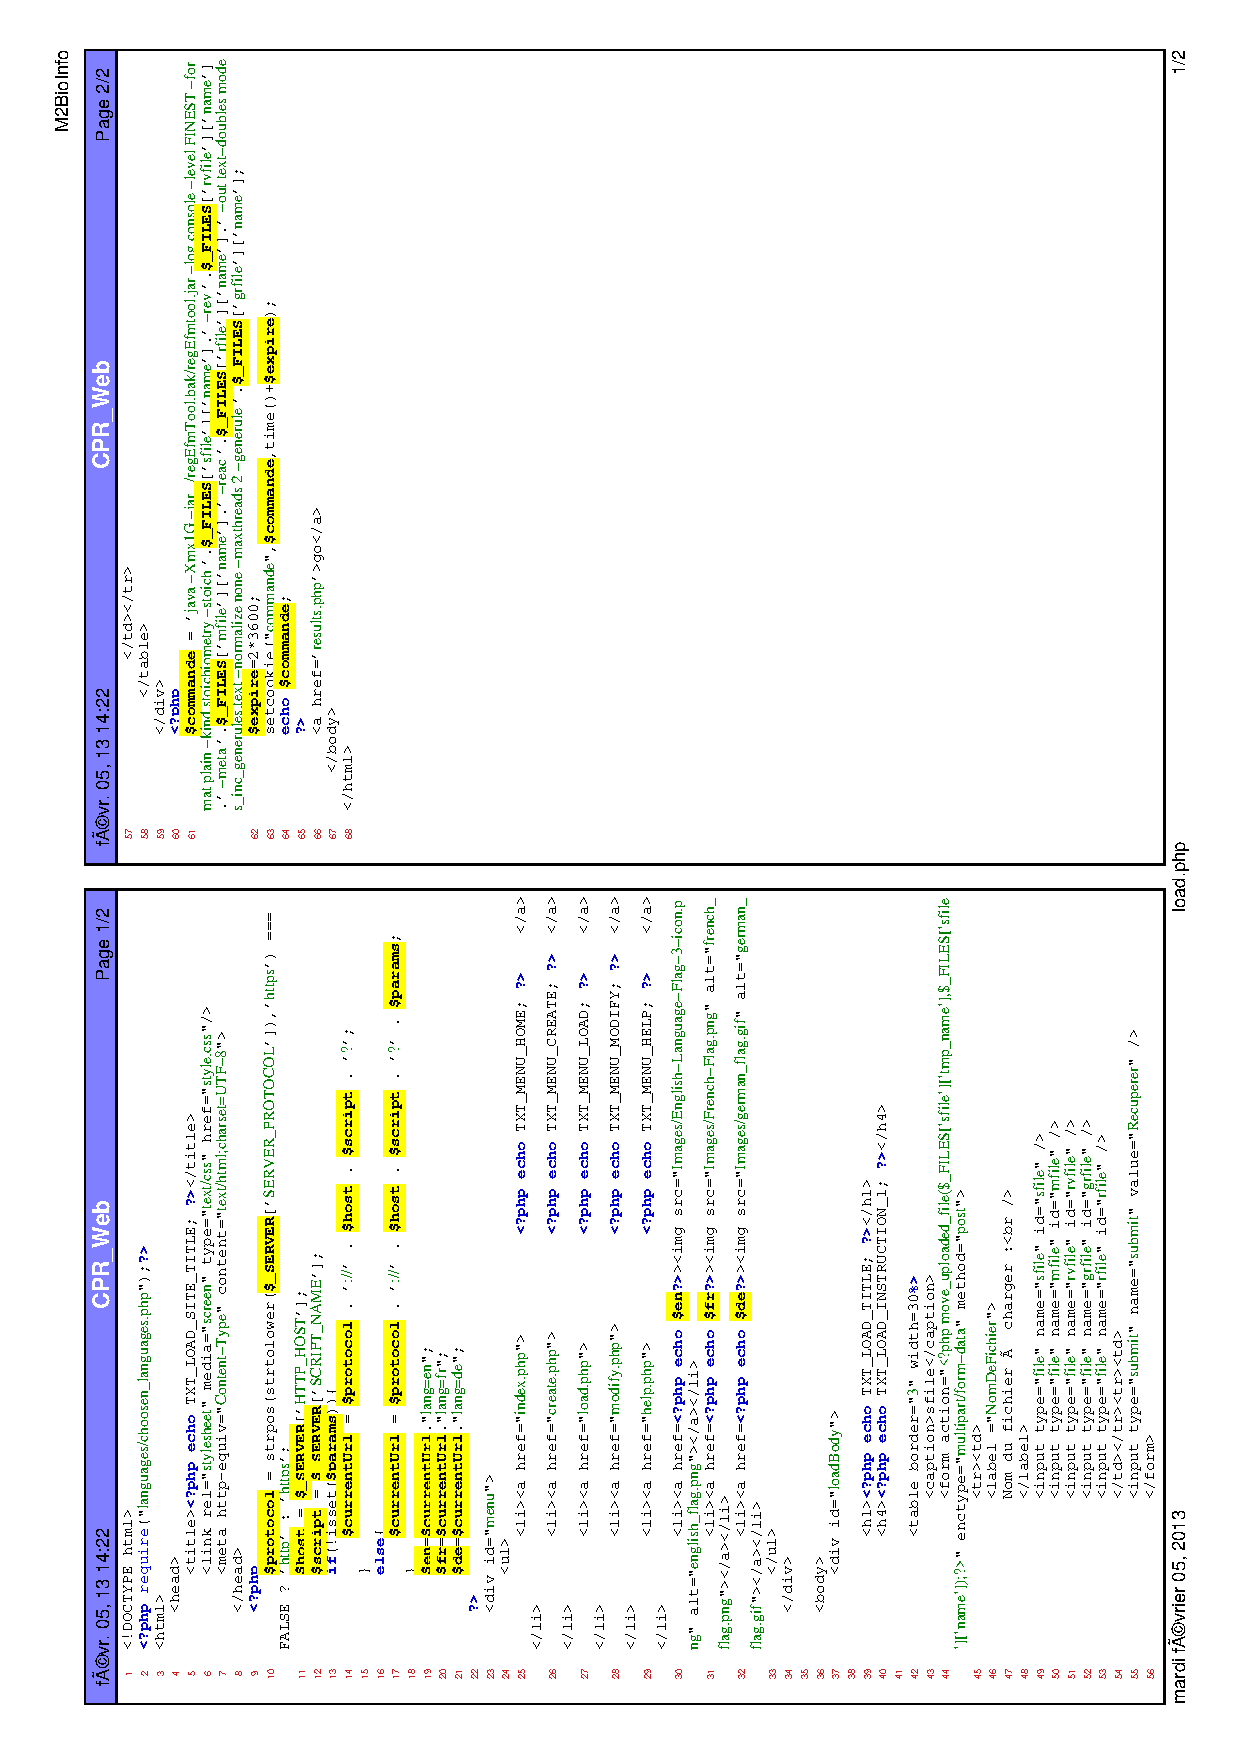
\includegraphics[width=0.90\textwidth]{../Images/Rapport/chargement.png}  
		 \end{minipage}}
		\caption{Partie de la page de chargement d'un réseau préexistant}
  		\label{chargement1}
  	\end{center}	
\end{figure}

L'utilisateur n'aura plus qu'à cliquer sur le bouton \textit{Étape suivante} pour générer le début de la ligne de commande. Tous les paramètres sauf ceux concernant les fichiers d'entrée seront alors récupérés. L'utilisateur est renvoyé sur une nouvelle page qui permet de charger ses fichiers depuis son disque dur et de lancer le logiciel. 

\subsection{Chargement des fichiers}
Cette page permet à l'utilisateur de sélectionner les fichiers à charger depuis son disque dur. Il y a un ordre précis du type des fichiers à charger (indiqué à l'utilisateur). 

%\begin{figure}[!ht]
%	\begin{center}
%		\fbox{
%   		 \begin{minipage}[c]{0.9\textwidth}
%  			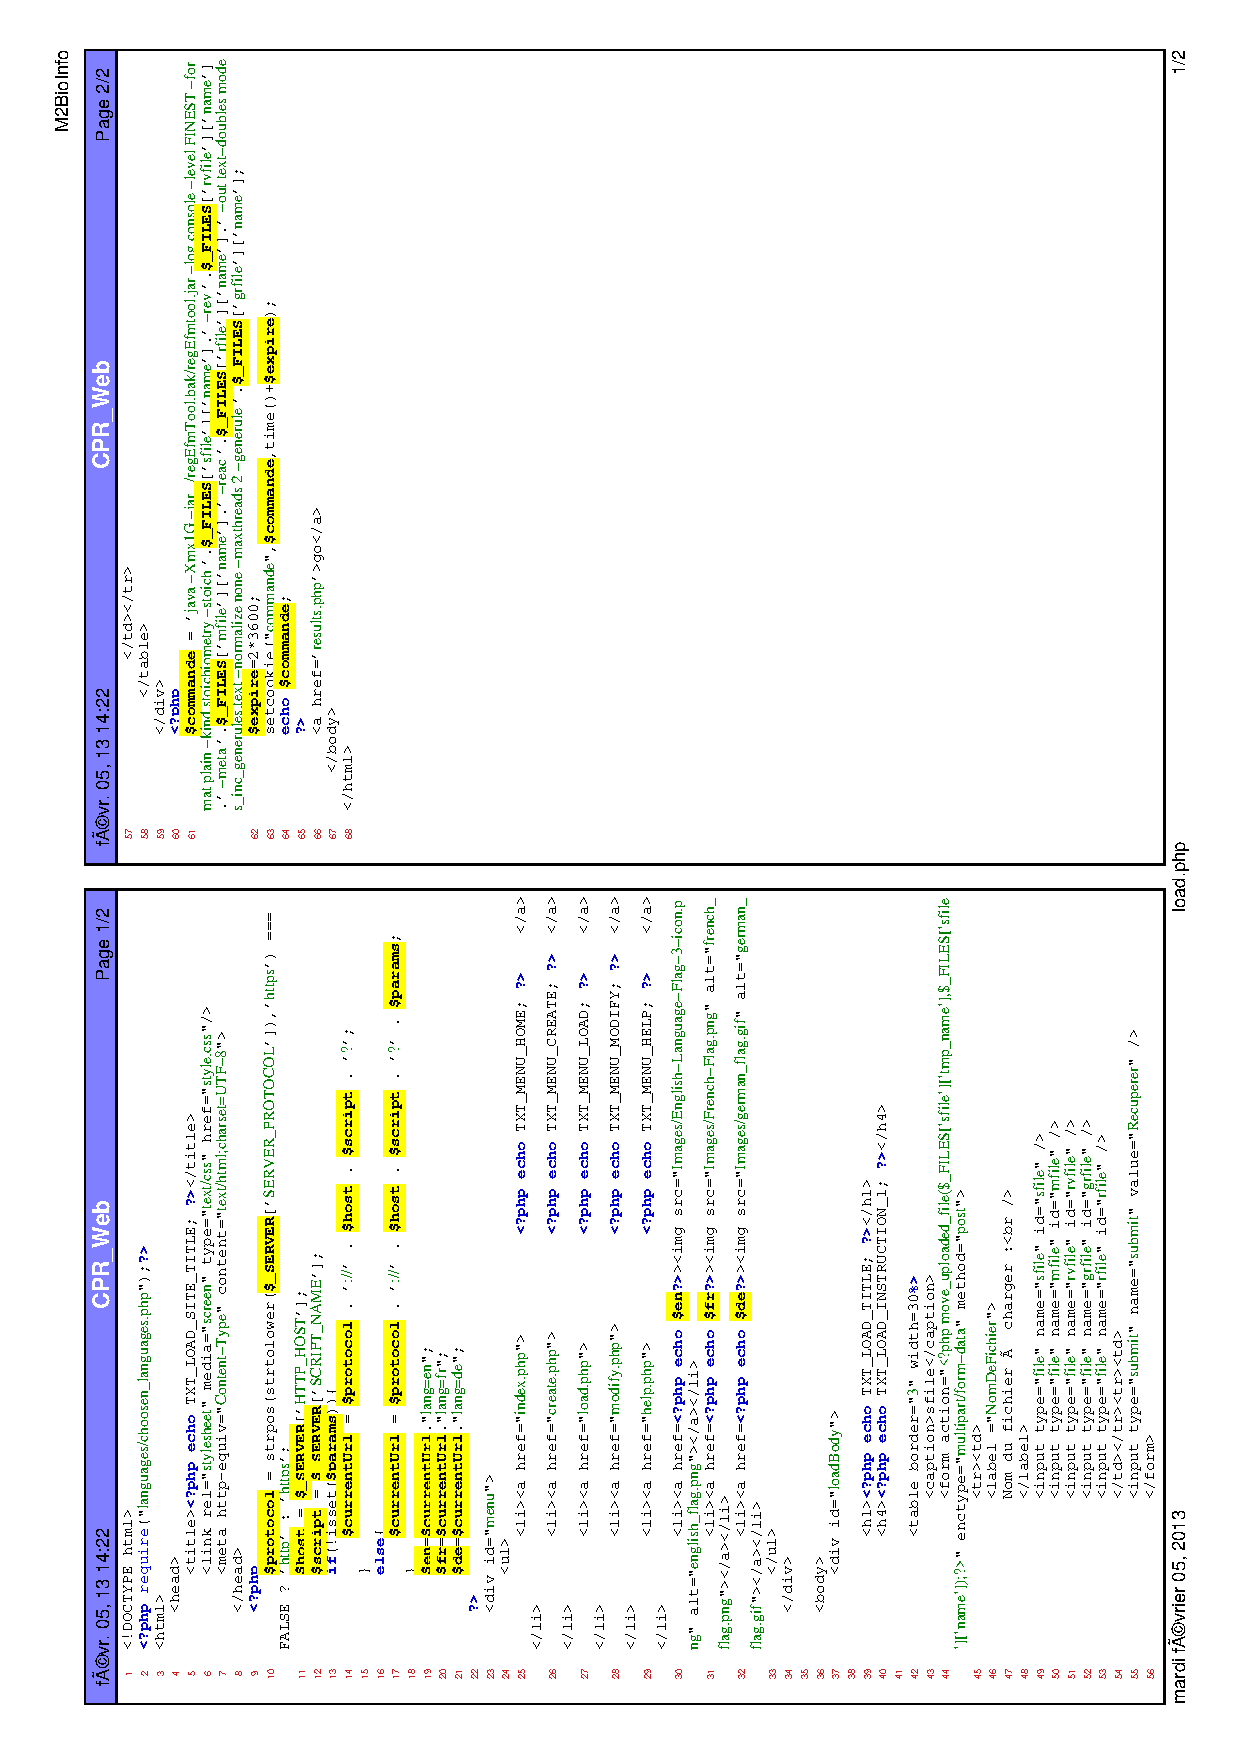
\includegraphics[width=0.90\textwidth]{../Images/Rapport/chargement.png}  
%		 \end{minipage}}
%		\caption{Partie de la page de chargement d'un réseau préexistant}
%  		\label{chargement2}
%  	\end{center}	
%\end{figure}

Une fois les fichiers sélectionnés, il suffit de cliquer sur \textit{Submit} pour effectuer le chargement.

%~~~~~~~~~~~~~~~~~~~~~~~~~~~~~
\section{Affichage des résultats}
%~~~~~~~~~~~~~~~~~~~~~~~~~~~~~

La page des résultats permet deux choses : l'exécution de regEfmtool et l'affichage des modes élémentaires, obtenus par le parse du fichier généré par l'exécution de regEfmtool.\\

Tout d'abord, la commande d'exécution de regEfmtool générée en partie depuis la page de choix des options est récupérée sur la page des résultats pour permettre son exécution.\\
L'exécution génère deux types de résultats : le fichier contenant les modes élémentaires ainsi que le log s'il est demandé.\\ 

Une fois l'exécution terminée, les résultats précédents seront affichés.\\
Les modes élémentaires sont affichés sous la forme d'un tableau contenant:
\begin{itemize}
\item En abscisse, les modes élémentaires obtenus
\item En ordonnée, toutes les réactions pouvant être impliquées\\
\end{itemize}

Cette page contient aussi trois boutons : 
\begin{itemize}
\item l'un permet de finir les calculs et de revenir à la page d'accueil,
\item le deuxième permet de revenir à la page d'accueil mais pour analyser un nouveau réseau et ainsi comparer les deux résultats générés, 
\item le troisième permet d'afficher l'outil de recherche sur le log et de sélectionner la catégorie que l'utilisateur veut afficher ou la totalité.\\
\end{itemize}

La page d'extraction des résultats offre à l'utilisateur la possibilité de visualiser l'ensemble des résultats généré par RegEfmetool ou de pouvoir extraire une partie de ces dernier à l'aide d'un mot clé selectionné dans le menu déroulant.

\begin{figure}[!ht]
	\begin{center}
		\fbox{
   		 \begin{minipage}[c]{0.9\textwidth}
  			\includegraphics[width=0.90\textwidth]{../Images/Rapport/extractionResultat.png}  
		 \end{minipage}}
		\caption{Page de recherche sur le log}
  		\label{chargement1}
  	\end{center}	
\end{figure}








 

%%%%%%%%%%%%%%%%%%%%%%%%%%%%%%
\chapter{Réalisation}
%%%%%%%%%%%%%%%%%%%%%%%%%%%%%%

%~~~~~~~~~~~~~~~~~~~~~~~~~~~~~
\section{Ergonomie de l'interface}
%~~~~~~~~~~~~~~~~~~~~~~~~~~~~~

\subsection{Mise en page}
Expliquer les div, le css ...

% Page d'options
Elle est composée d'un emboîtement de plusieurs sections, grâce à la balise HTML  \texttt{<div>}, qui est une sorte de conteneur. Comme nous l'avons précisé précédemment, nous avons séparé les options en plusieurs catégories et sous-catégories. 

\subsection{Langues}
...

%~~~~~~~~~~~~~~~~~~~~~~~~~~~~~
\section{Création d'un nouveau réseaux}
%~~~~~~~~~~~~~~~~~~~~~~~~~~~~~

\subsection{Initialisation des fichiers}
La création d'un nouveau réseaux dans WRET se fait via la page \emph{create.php}.
A partir de cette page l'utilisateur doit dans un premier temps appuyer sur le bouton \emph{Initialiser les fichiers} (Figure \ref{boutonInit}) s'il désire initialiser ses fichiers. 

\begin{figure}[!ht]
	\begin{center}
		\fbox{
   		 \begin{minipage}[c]{0.5\textwidth}
  			\includegraphics[width=0.90\textwidth]{../Images/Rapport/creation1-1.png}  
		 \end{minipage}}
		\caption{Bouton d'initialisation des fichiers}
  		\label{boutonInit}
  	\end{center}	
\end{figure}

Ce bouton appelle le fichier \emph{initfiles.php} qui va créer les 11 fichiers nécessaires à la mise en place d'un nouveau réseau.\\
Dans ces fichiers, nous trouvons des fichiers qui seront utilisés dans le lancement de \emph{regEfmtool} (rfile, mfile, rvfile, sfile) et également des fichiers temporaires (\emph{irrevTemp}, \emph{revTemp}, \emph{reactionTemp.txt}, \emph{reactionTemp2.txt}, \emph{matrice.txt} ou encore \emph{matrice2.txt} ainsi que la base du fichier au format \emph{DAT}).\\
Tous ces fichiers sont donc créés et donnent les droits d'édition, de lecture et d'exécution à tous les utilisateurs pour ces fichiers, afin de pouvoir être modifiés sur le serveur.

\subsection{Réactions et réversibilité}
Sous la touche \emph{Initialiser les fichiers} de la page \emph{create.php}, une fenêtre de texte permet de rentrer les réactions du réseau métabolique une à une ainsi que la réversibilité de la réaction (Figure \ref{boutonAjout}). 

\begin{figure}[!ht]
	\begin{center}
		\fbox{
   		 \begin{minipage}[c]{0.7\textwidth}
  			\includegraphics[width=0.90\textwidth]{../Images/Rapport/creation1-2.png}  
		 \end{minipage}}
		\caption{Bouton d'ajout d'une réaction}
  		\label{boutonAjout}
  	\end{center}	
\end{figure}

Si l'utilisateur oublie de cocher la réversibilité de la réaction et clique sur \emph{Ajouter}, un message d'erreur s'affichera et empêchera le passage à l'étape suivante. Les réactions doivent être enregistrées par l'utilisateur en respectant la syntaxe des fichier au format \emph{DAT}. Ces informations vont alors être envoyées au fichier \emph{createFiles.php}, via le bouton \emph{Ajouter}.\\
Ce fichier redirige vers différentes pages, dans l'ordre : \emph{reac.php}, \emph{parser\_enzyme.php}, \emph{parser\_reversibility.php}, \emph{parser\_metabolite.php}, \emph{parser\_stoechiometry.php}.
La première page \emph{reac.php} va permettre d'écrire dans un fichier temporaire (reactionTemp.txt) les réactions, et également, de sauvegarder la réversibilité de la réaction (0 pour non réversible, et 1 pour réversible).\\
L'ordre est ainsi conservé entre les réactions et leur réversibilité.

\subsection{Nom de réactions : enzymes}
Une fois les données de réactions et de réversibilité enregistrées, la page \emph{parser\_enzymes.php} est appelée. Elle va parser le fichier temporaire des réactions (\emph{reactionTemp.txt}) et va extraire le premier élément de la réaction situé avant le ":", qui se trouve être le nom de la réaction (nom de l'enzyme généralement).\\
Ces noms sont enregistrés dans un fichier (\emph{reaction.rfile}) en respectant les espaces et la syntaxe nécessaire à l'utilisation au sein de \emph{regEfmtool}.

\subsection{Métabolites}
Après enregistrements des enzymes, le fichier \emph{parser\_metabolites.php} est appelé. Ce script va parser le fichier temporaire contenant les réactions (\emph{reactionTemp.txt}) et va enregistrer chacun des métabolites dans un fichier (\emph{meatbolites.mfile}). Au cours de ce parsage, seuls les éléments situés après le nom de l'enzyme seront pris en compte. Les noms présents plusieurs fois dans le fichier de réactions sont enregistrés une seule fois dans le fichier \emph{metabolites.mfile}.

\subsection{Stœchiométrie}
Enfin après génération des fichiers: \emph{rvfile}, \emph{mfile}, \emph{sfile}, \emph{rfile}, le script \emph{parser\_stoechiometry} est appelé. Il va lancer le script \emph{parser\_stoechiometry.py}. Ce dernier permet de générer la matrice de stœchiométrie nécessaire a \emph{regEfmtool}. Pour ce faire, il prend les fichiers \emph{reactionTemp.txt} et \emph{metabolites.mfile} en entrée. Il génère la matrice ligne par ligne (une ligne correspondant à une réaction). \\
Pour chaque ligne du fichier \emph{reactionTemp.txt} une liste est créée et, pour chaque métabolite de cette réaction, sa stœchiométrie est enregistrée en respectant son ordre dans le fichiers contenant les réactifs. Ce script fournit alors en sortie le fichier \emph{stoechiometry.sfile}.

\subsection{Modification du réseaux}
Une fois les fichiers générés l'utilisateur est redirigé sur la page \emph{create.php}.
Sous la touche \emph{Ajouter} se trouve une zone de texte (Figure \ref{boutonAjout}) où l'utilisateur peut modifier un réseau déjà rentré. 

\begin{figure}[!ht]
	\begin{center}
		\fbox{
   		 \begin{minipage}[c]{0.7\textwidth}
  			\includegraphics[width=0.90\textwidth]{../Images/Rapport/creation1-3.png}  
		 \end{minipage}}
		\caption{Bouton de modification}
  		\label{boutonModif}
  	\end{center}	
\end{figure}

En effet cette zone appelle le fichier \emph{reactionTemp.txt} et permet la modification de son contenu (pour corriger une erreur de frappe notamment). Cette zone de texte va appeler la page \emph{modifier.php} lors de l'utilisation du bouton \emph{Modifier}.\\
 Cette page efface le précédant fichier \emph{reactionTemp.txt} et insère le nouveau contenu que l'utilisateur a modifié. \\
 Les fichiers \emph{metabolites.mfile}, \emph{stoechiometry.sfile}, \emph{reactions.rfile}, \emph{reversibility}, sont également générés à nouveau, à chaque modification du fichier \emph{reactionTemp.txt}.
 
\subsection{Création du fichier \emph{DAT}}
Sous la zone de texte modifiable, un bouton \emph{DAT} permet de générer un fichier au format \emph{DAT} du réseaux métabolique précédemment rentré. \\

\begin{figure}[!ht]
	\begin{center}
		\fbox{
   		 \begin{minipage}[c]{0.3\textwidth}
  			\includegraphics[width=0.90\textwidth]{../Images/Rapport/creation2-1.png}  
		 \end{minipage}}
		\caption{Bouton de création du fichier au format \emph{DAT}}
  		\label{boutonDAT}
  	\end{center}	
\end{figure}

Ce bouton (Figure \ref{boutonDAT}) appelle la page \emph{finish\_files.php} qui va concaténer trois fichiers :
\begin{itemize}
\item \emph{irrevTemp.txt}
\item \emph{revTemp.txt}
\item \emph{reactiontemp2.txt}
\end{itemize}
Le premier fichier contient l'ensemble des enzymes catalysant les réactions irréversibles. Le second contient l'ensemble des enzymes catalysant des réactions réversibles, et enfin le dernier fichier contient l'ensemble des réactions du réseaux. \\
Chacun de ces fichiers contient les balises \emph{-IRREV}, \emph{-REV}, \emph{-CAT}, selon son contenu et respecte la syntaxe propre au format \emph{DAT}.

%~~~~~~~~~~~~~~~~~~~~~~~~~~~~~
\section{Règles des gènes}
%~~~~~~~~~~~~~~~~~~~~~~~~~~~~~

La page permettant la saisie des règles générales est obtenue à l'aide du fichier \emph{generules.php}.\\
L'affichage à l'ouverture de la page n'est composé que d'une zone de texte et d'un bouton \emph{Ok} (Figure \ref{boutonOK}) qui est de type \textit{submit}. 

\begin{figure}[!ht]
	\begin{center}
		\fbox{
   		 \begin{minipage}[c]{0.3\textwidth}
  			\includegraphics[width=0.90\textwidth]{../Images/Rapport/generules-1.png}  
		 \end{minipage}}
		\caption{Bouton du choix du nombre de réactions pour une règle}
  		\label{boutonOK}
  	\end{center}	
\end{figure}

Au clic, ce bouton fait appel à la fonction \emph{add\_reaction()} qui créée  deux menus déroulants (pour la première et la dernière, Figure \ref{menusDeroulants1}) ou trois menus déroulants (pour les autres, Figure \ref{menusDeroulants2}) par réaction jusqu'à atteindre le nombre de réactions entrées par l'utilisateur. 

\begin{figure}[!ht]
	\begin{center}
		\fbox{
   		 \begin{minipage}[c]{0.7\textwidth}
  			\includegraphics[width=0.90\textwidth]{../Images/Rapport/generules-2.png}  
		 \end{minipage}}
		\caption{Menus déroulant si 2 réactions dans la règle}
  		\label{menusDeroulants1}
  	\end{center}	
\end{figure}

\begin{figure}[!ht]
	\begin{center}
		\fbox{
   		 \begin{minipage}[c]{0.8\textwidth}
  			\includegraphics[width=0.90\textwidth]{../Images/Rapport/generules-3.png}  
		 \end{minipage}}
		\caption{Menus déroulant si 3 réactions dans la règle}
  		\label{menusDeroulants2}
  	\end{center}	
\end{figure}

Elle vérifie également que le nombre de réactions entrées par l'utilisateur est au moins égal à 2, sinon elle affiche un message sous la forme d'une alerte à l'utilisateur.\\
Les réactions sont récupérées à partir de \emph{reactions.rfile}.\\

L'utilisateur peut sélectionner plusieurs fois la m\^eme réaction dans sa règle, sauf pour le choix de la dernière (ligne THEN). Cette particularité est gérée par la fonction \texttt{choice(form, val)}. Celle-ci permet de remplir les menus déroulants quand une réaction a été choisie et pour la dernière seules les réactions non sélectionnées précédemment appara\^issent.

Lorsque l'utilisateur a choisi toutes ses réactions, leur opérateur et leur valeur, il clique sur le bouton \emph{Ajouter}. Celui-ci fait appel à la fonction \texttt{validateForm()} qui vérifie que tous les champs ont bien été sélectionnés. Si la fonction retourne VRAI, il fait appel au fichier \emph{createGrfile.php} qui écrit la règle dans le fichier \emph{grfile.txt}.\\
Le fichier \emph{createGrfile.php} écrit dans le fichier \emph{grfile} selon certaines règles. En effet, l'écriture de la règle dépend des valeurs associées aux réactions et des opérateurs choisis.\\

Si la valeur de la réaction qui suit le "THEN" est 0, alors il y aura le symbole "!" au début de la règle (juste après le "="), sauf si la règle ne contient que deux réactions.\\
Si les autres réactions ont pour valeur:
\begin{itemize}
\item 0, alors on écrira (!0reac)
\item 1, alors on écrira (!1reac)
\item f, alors on écrira (!freac)
\end{itemize}
En revanche, si la valeur de la réaction après "THEN" est 1, les autres réactions s'écriront:
\begin{itemize}
\item 0reac si sa valeur est 0
\item 1reac si sa valeur est 1
\item freac si sa valeur est f
\end{itemize}
De plus, si l'opérateur "AND" est sélectionné il sera écrit sous la forme \& dans le fichier, l'opérateur "OR" sera lui écrit $|$. Quand la règle est composée d'au moins trois réactions, des parenthèses sont ajoutées après chaque réaction sauf la première et la dernière. Des parenthèses entourent l'ensemble des réactions situées après le "=".\\

Pour mieux comprendre l'écriture du fichier \emph{generules.grfile}, voici un exemple:\\

Choix de l'utilisateur sur la page Web: \\
\begin{DDbox}{\linewidth}
\begin{lstlisting}
IF reaction: R1 valeur: 1
Operateur: AND reaction: R2 valeur: 0
Operateur: OR reaction: R3 valeur: 0
THEN reaction: R4 valeur: 0
\end{lstlisting}
\end{DDbox}

Règle écrite dans le fichier: \\
\begin{DDbox}{\linewidth}
\begin{lstlisting}
R4 = (!((1R1 \& (!0R2)) $|$ (!0R3))
\end{lstlisting}
\end{DDbox}


%~~~~~~~~~~~~~~~~~~~~~~~~~~~~~
\section{Choix des options de lancement}
%~~~~~~~~~~~~~~~~~~~~~~~~~~~~~

La page permettant la sélection des options de lancement est obtenue à l'aide du fichier \emph{options.php}. Comme nous l'avons dit précédemment, nous avons séparé les options en une série de catégories et sous catégories, le tout contenu dans un formulaire afin de gérer l'interaction avec l'utilisateur. Ce dernier peut sélectionner les options qu'il désire avec une combinaison de \textit{radioboutons} et de zones de texte. Les \textit{radioboutons} d'une même sous-section ont le même attribut \textit{name} afin de ne pouvoir en sélectionner qu'un seul. \\

Prenons comme exemple la première sous catégorie (Figure \ref{affichageResults}) :

\begin{figure}[!ht]
	\begin{center}
		\fbox{
   		 \begin{minipage}[c]{0.3\textwidth}
  			\includegraphics[width=0.90\textwidth]{../Images/Rapport/options-1.png}  
		 \end{minipage}}
		\caption{Sous catégorie d'affichage des résultats dans la catégorie d'enregistrement}
  		\label{affichageResults}
  	\end{center}	
\end{figure}

Voici le code HTML/PHP qui correspond :

\scriptsize
\begin{DDbox}{\linewidth}
\begin{lstlisting}
<input type="radio" name="choix1" value="log console" checked="checked">	<?php echo TXT_OPTIONS_SAVING_3; ?> 
<input type="radio" name="choix1" value="log file"> <?php echo TXT_OPTIONS_SAVING_4; ?> 
<?php echo TXT_OPTIONS_SAVING_5; ?> <input type="text"	 name="log_nomFichier" 	size="10" id="texte1">
\end{lstlisting}
\end{DDbox}

\normalsize

Le premier \textit{radiobouton} est pré-coché avec l'attribut \textit{checked="checked"} afin de guider l'utilisateur. Si cette option ne lui contient pas, il lui suffit de cocher le deuxième \textit{radiobouton} et de remplir la zone de texte associée. \\

Ce sont les attributs \textit{value} de ces boutons qui sont récupérés avec un script JavaScript. Ce dernier, nommé \emph{choixOptions.js}, permet de vérifier quels \textit{radioboutons} sont cochés et récupère ce qu'il a dans l'attribut \textit{value} de ceux-ci quand c'est le cas. Il est appelé lors du clic sur le bouton \textit{Lancement} en bas de la page. De plus, c'est dans ce script qu'est générée la commande qui permettra le lancement de regEfmtool. Elle est contenue dans une variable nommée  \textit{commande}, qui se remplit des paramètres sélectionnés. \\

Exemple du code JavaScript qui permet la récupération des \textit{values} précédentes : \\

\begin{DDbox}{\linewidth}
\begin{lstlisting}
var commande = "java -Xmx1G -jar ../regEfmtool.jar";

  // SAVE
  // Display
  if (formulaire.choix1[0].checked) { 
    valeur1 = " -" + formulaire.choix1[0].value; 
    commande = commande + valeur1;
  }
  else if (formulaire.choix1[1].checked) { 
    var nom1 = document.getElementById('texte1').value;
    valeur1 = " -" + formulaire.choix1[1].value + " " + nom1; 
    commande = commande + valeur1;
  }
\end{lstlisting}
\end{DDbox}

La variable \textit{commande} est une chaîne de caractères qui contient le début de la commande Java. Les paramètres sont ensuite ajoutés au fur et à mesure de la vérification de la sélection des boutons. \\

Cette commande est envoyée via un \textit{cookie} à la page d'affichage des résultats pour le lancement de regEfmtool. 

%~~~~~~~~~~~~~~~~~~~~~~~~~~~~~
\section{Chargement d'un réseau pré-existant}
%~~~~~~~~~~~~~~~~~~~~~~~~~~~~~

Ce sont les pages \emph{load.php} et \emph{load\_files.php} qui permettent le chargement des fichiers contenant un réseau pré-existant depuis le disque dur de l'utilisateur. Tout d'abord, la page \emph{load.php} permet à ce dernier de choisir les paramètres de la commande de lancement de regEfmtool, de le même façon que pour la page \emph{options.php}. Cependant, la deuxième grande catégorie diffère car le choix des fichiers à charger se fera lors d'une étape ultérieure. Ici, l'utilisateur coche les options qu'il désire et clique sur le bouton "Étape suivante". Ce bouton fait appel au script JavaScript \emph{actioLoad.js}, qui fonctionne sur le même principe que \emph{choixOptions.js}. \\

Ensuite, l'utilisateur est dirigé vers la page \emph{load\_files.php} 

%~~~~~~~~~~~~~~~~~~~~~~~~~~~~~
\section{Affichage des résultats}
%~~~~~~~~~~~~~~~~~~~~~~~~~~~~~






\bibliographystyle{unsrt}
\bibliography{rapport}


\end{document}